% Chapter 3: Probability and Information Theory

\chapter{Probability and Information Theory}
\label{chap:probability}

This chapter introduces fundamental concepts from probability theory and information theory that are essential for understanding machine learning and deep learning. Topics include probability distributions, conditional probability, expectation, variance, entropy, and mutual information.

\section*{Learning Objectives}

After studying this chapter, you will be able to:

\begin{itemize}
    \item \textbf{Understand probability foundations}: Grasp the intuitive meaning of probability distributions, both discrete and continuous, and how they model uncertainty in real-world scenarios.
    
    \item \textbf{Apply conditional probability}: Use Bayes' theorem to update beliefs with new evidence and understand its central role in machine learning algorithms.
    
    \item \textbf{Calculate statistical measures}: Compute expectation, variance, and covariance to characterize the behavior of random variables and their relationships.
    
    \item \textbf{Work with common distributions}: Recognize when to use Bernoulli, Gaussian, and other probability distributions in machine learning contexts.
    
    \item \textbf{Quantify information content}: Use entropy, cross-entropy, and KL divergence to measure uncertainty and information in data and models.
    
    \item \textbf{Apply information theory}: Connect information-theoretic concepts to loss functions, model selection, and representation learning in deep neural networks.
\end{itemize}

% Chapter 3, Section 1: Probability Distributions

\section{Probability Distributions \difficultyInline{beginner}}
\label{sec:probability-distributions}

Probability distributions are mathematical functions that describe how probabilities are distributed across different possible outcomes of a random variable, providing the fundamental framework for modeling uncertainty in data and making predictions in machine learning and deep learning applications.

\subsection{Intuition: What is Probability?}

Imagine you're playing a game of dice where you roll a standard six-sided die with numbers 1 through 6. Before rolling, you know that each face has an equal chance of appearing, meaning that if you roll the die many times, each number will appear approximately one-sixth of the time. This "chance" is what we call probability - a number between 0 and 1 that quantifies how likely an event is to occur, where 0 means impossible and 1 means certain. In machine learning, we face uncertainty everywhere, from data uncertainty about whether the next customer will click on an ad, to model uncertainty about how confident our neural network is in its prediction, to parameter uncertainty about what the best value is for our model's weights. Probability distributions are mathematical tools that help us model and work with this uncertainty systematically, providing a rigorous framework for making decisions under uncertainty and quantifying the confidence we can have in our predictions and model parameters.

\subsection{Visualizing Probability}

Consider a simple example: predicting whether it will rain tomorrow. We might say there's a 30\% chance of rain, which means that if we could repeat tomorrow 100 times, rain would occur about 30 times, the probability of rain is 0.3, and the probability of no rain is 0.7. This intuitive understanding of probability helps us visualize how probability distributions work - they assign numerical values to different outcomes, showing us not just what can happen, but how likely each outcome is to occur.

\begin{figure}[h]
\centering
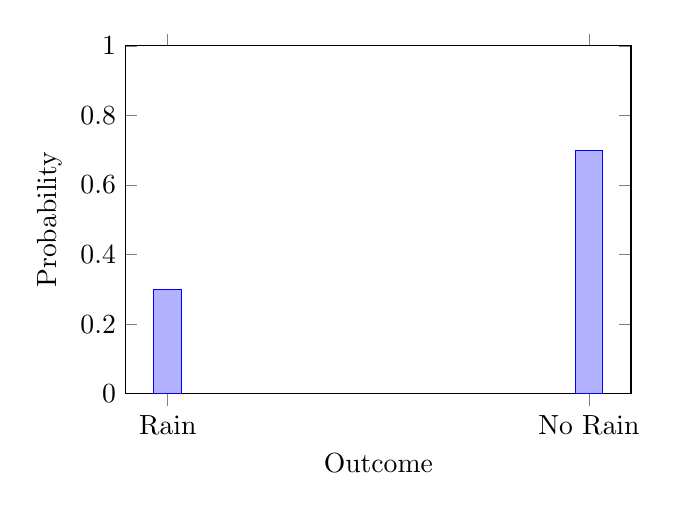
\begin{tikzpicture}
\begin{axis}[
    ybar,
    ylabel={Probability},
    xlabel={Outcome},
    xtick={1,2},
    xticklabels={Rain, No Rain},
    ymin=0,
    ymax=1,
    width=8cm,
    height=6cm
]
\addplot coordinates {(1,0.3) (2,0.7)};
\end{axis}
\end{tikzpicture}
\caption{Probability distribution for rain prediction}
\label{fig:rain-probability}
\end{figure}

Probability theory provides a mathematical framework for quantifying uncertainty. In deep learning, we use probability distributions to model uncertainty in data, model parameters, and predictions.

\subsection{Discrete Probability Distributions}

Discrete probability distributions deal with outcomes that can be counted and listed explicitly, such as coin flips with heads or tails, dice rolls with numbers 1 through 6, or email classification with spam or not spam. These distributions assign probabilities to each possible outcome, where the sum of all probabilities equals 1, representing the fact that one of the possible outcomes must occur.

A discrete random variable $X$ takes values from a countable set. The \textbf{probability mass function} (PMF) $P(X=x)$ assigns probabilities to each possible value:

\begin{equation}
P(X=x) \geq 0 \quad \text{for all } x
\end{equation}

\begin{equation}
\sum_{x} P(X=x) = 1
\end{equation}

\subsubsection{Example: Fair Coin}

For a fair coin, we have:
\begin{align}
P(X=0) &= 0.5 \quad \text{(Tails)} \\
P(X=1) &= 0.5 \quad \text{(Heads)}
\end{align}

\begin{figure}[h]
\centering
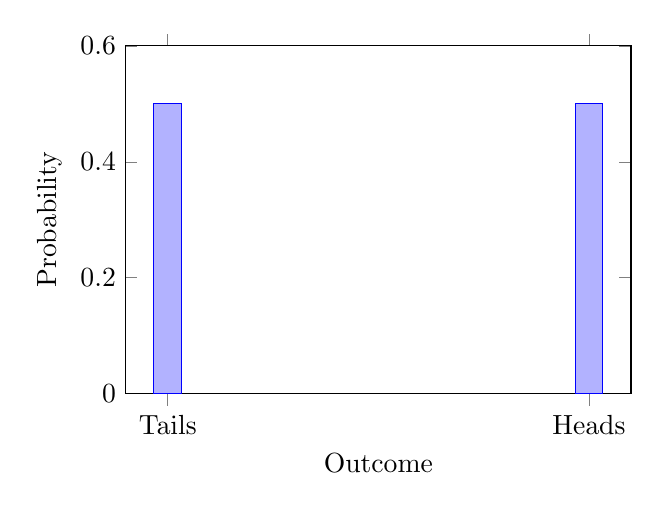
\begin{tikzpicture}
\begin{axis}[
    ybar,
    ylabel={Probability},
    xlabel={Outcome},
    xtick={0,1},
    xticklabels={Tails, Heads},
    ymin=0,
    ymax=0.6,
    width=8cm,
    height=6cm
]
\addplot coordinates {(0,0.5) (1,0.5)};
\end{axis}
\end{tikzpicture}
\caption{Probability mass function for a fair coin}
\label{fig:coin-pmf}
\end{figure}

\subsection{Continuous Probability Distributions}

Continuous probability distributions deal with variables that can take any value within a continuous range, such as the height of people which can be 170 cm, 170.5 cm, 170.52 cm, and so on, or temperature which can be 22.3°C, 22.34°C, 22.341°C, and so on, or neural network weights which can be 0.1234, 0.12345, 0.123456, and so on. Since there are infinitely many possible values, we can't assign probabilities to individual points, but instead use density functions that describe how "concentrated" the probability is in different regions of the continuous space.

A continuous random variable can take any value in a continuous range. We describe it using a \textbf{probability density function} (PDF) $p(x)$:

\begin{equation}
p(x) \geq 0 \quad \text{for all } x
\end{equation}

\begin{equation}
\int_{-\infty}^{\infty} p(x) \, dx = 1
\end{equation}

The probability that $X$ falls in an interval $[a, b]$ is:

\begin{equation}
P(a \leq X \leq b) = \int_a^b p(x) \, dx
\end{equation}

\subsubsection{Example: Normal Distribution}

The most common continuous distribution is the \textbf{normal (Gaussian) distribution}, which looks like a bell curve:

\begin{figure}[h]
\centering
\begin{tikzpicture}
\begin{axis}[
    ylabel={Probability Density},
    xlabel={Value},
    domain=-3:3,
    width=10cm,
    height=6cm,
    samples=100
]
\addplot[bookpurple, thick] {1/sqrt(2*pi) * exp(-x^2/2)};
\addplot[bookred, thick] {1/sqrt(2*pi*0.5) * exp(-(x-0.5)^2/(2*0.5))};
\end{axis}
\end{tikzpicture}
\caption{Two normal distributions with different means and standard deviations}
\label{fig:normal-distributions}
\end{figure}

The area under the curve between any two points gives the probability of the variable falling in that range.

\subsection{Joint and Marginal Distributions}

In real-world scenarios, we often deal with multiple variables simultaneously, such as weather prediction involving both temperature and humidity, image classification involving pixel values at different positions, or stock prices involving multiple stocks in a portfolio. The joint distribution tells us about the probability of combinations of values across all variables, while marginal distributions tell us about individual variables when we ignore the others, providing a way to understand both the relationships between variables and the behavior of individual variables in isolation.

\subsubsection{Example: Weather Data}

Consider a simple weather dataset with two variables:
\begin{itemize}
    \item $X$: Temperature (Hot/Cold)
    \item $Y$: Humidity (High/Low)
\end{itemize}

\begin{table}[h]
\centering
\begin{tabular}{|c|c|c|c|}
\hline
 & $Y=$ High & $Y=$ Low & \textbf{Marginal} \\
\hline
$X=$ Hot & 0.3 & 0.2 & \textbf{0.5} \\
$X=$ Cold & 0.1 & 0.4 & \textbf{0.5} \\
\hline
\textbf{Marginal} & \textbf{0.4} & \textbf{0.6} & \textbf{1.0} \\
\hline
\end{tabular}
\caption{Joint probability table for weather data}
\label{tab:weather-joint}
\end{table}

For multiple random variables $X$ and $Y$, the \textbf{joint distribution} $P(X, Y)$ describes their combined behavior. The \textbf{marginal distribution} is obtained by summing (or integrating) over the other variable:

\begin{equation}
P(X=x) = \sum_{y} P(X=x, Y=y)
\end{equation}

For continuous variables:

\begin{equation}
p(x) = \int p(x, y) \, dy
\end{equation}

From our weather example:
\begin{itemize}
    \item $P(X=\text{Hot}) = 0.3 + 0.2 = 0.5$ (marginal probability of hot weather)
    \item $P(Y=\text{High}) = 0.3 + 0.1 = 0.4$ (marginal probability of high humidity)
\end{itemize}

% Chapter 3, Section 2: Conditional Probability and Bayes' Rule

\section{Conditional Probability and Bayes' Rule \difficultyInline{beginner}}
\label{sec:conditional-probability}

\subsection{Intuition: Updating Beliefs with New Information}

Imagine you're a doctor trying to diagnose a patient. Initially, you might think there's a 5\% chance the patient has a rare disease. But then the patient tells you they have a specific symptom that's present in 80\% of people with that disease. How should you update your belief?

This is exactly what \textbf{conditional probability} helps us do - it tells us how to update our beliefs when we get new information.

\subsection{Conditional Probability}

The \textbf{conditional probability} of $X$ given $Y$ is:

\begin{equation}
P(X|Y) = \frac{P(X, Y)}{P(Y)}
\end{equation}

This quantifies how the probability of $X$ changes when we know the value of $Y$.

\subsubsection{Example: Medical Diagnosis}

Let's make this concrete with our medical example:
\begin{itemize}
    \item $D$: Patient has the disease (1 = yes, 0 = no)
    \item $S$: Patient has the symptom (1 = yes, 0 = no)
\end{itemize}

From medical records, we know:
\begin{itemize}
    \item $P(D=1) = 0.05$ (5\% of population has the disease)
    \item $P(S=1|D=1) = 0.8$ (80\% of diseased patients have the symptom)
    \item $P(S=1|D=0) = 0.1$ (10\% of healthy patients have the symptom)
\end{itemize}

If a patient has the symptom, what's the probability they have the disease?

Using Bayes' theorem (which we'll derive next):
\begin{align}
P(D=1|S=1) &= \frac{P(S=1|D=1)P(D=1)}{P(S=1)} \\
&= \frac{0.8 \times 0.05}{0.8 \times 0.05 + 0.1 \times 0.95} \\
&= \frac{0.04}{0.04 + 0.095} \\
&= \frac{0.04}{0.135} \approx 0.296
\end{align}

So even with the symptom, there's only about a 30\% chance the patient has the disease!

\subsection{Independence}

\subsubsection{Intuition: When Variables Don't Affect Each Other}

Two events are \textbf{independent} if knowing one doesn't change our belief about the other. For example:
\begin{itemize}
    \item \textbf{Independent}: Rolling two dice - the result of the first die doesn't affect the second
    \item \textbf{Dependent}: Weather and clothing choice - knowing it's raining affects the probability you'll wear a raincoat
\end{itemize}

Two random variables $X$ and $Y$ are \textbf{independent} if:

\begin{equation}
P(X, Y) = P(X)P(Y)
\end{equation}

Equivalently, $P(X|Y) = P(X)$ and $P(Y|X) = P(Y)$.

\subsubsection{Example: Independent vs Dependent Variables}

Consider two scenarios:

\textbf{Scenario 1 (Independent):} Flipping two coins
\begin{itemize}
    \item $P(\text{First coin = Heads}) = 0.5$
    \item $P(\text{Second coin = Heads}) = 0.5$
    \item $P(\text{Both Heads}) = 0.5 \times 0.5 = 0.25$ \checkmark
\end{itemize}

\textbf{Scenario 2 (Dependent):} Drawing cards without replacement
\begin{itemize}
    \item $P(\text{First card = Ace}) = 4/52 = 1/13$
    \item $P(\text{Second card = Ace}) = 3/51$ (if first was Ace) or $4/51$ (if first wasn't Ace)
    \item The probability of the second card depends on what the first card was
\end{itemize}

\subsection{Bayes' Theorem}

\subsubsection{Intuition: The Most Important Formula in Machine Learning}

Bayes' theorem is like a "belief update machine." It tells us how to revise our initial beliefs (prior) when we observe new evidence, to get our updated beliefs (posterior).

\textbf{Bayes' theorem} is fundamental to probabilistic inference:

\begin{equation}
P(X|Y) = \frac{P(Y|X)P(X)}{P(Y)}
\end{equation}

\subsubsection{Understanding Each Component}

In machine learning terminology:
\begin{itemize}
    \item $P(X)$ is the \textbf{prior} probability - what we believed before seeing the data
    \item $P(Y|X)$ is the \textbf{likelihood} - how likely the data is given our hypothesis
    \item $P(X|Y)$ is the \textbf{posterior} probability - what we believe after seeing the data
    \item $P(Y)$ is the \textbf{evidence} or marginal likelihood - the probability of observing the data
\end{itemize}

\subsubsection{Visualizing Bayes' Theorem}

\begin{figure}[h]
\centering
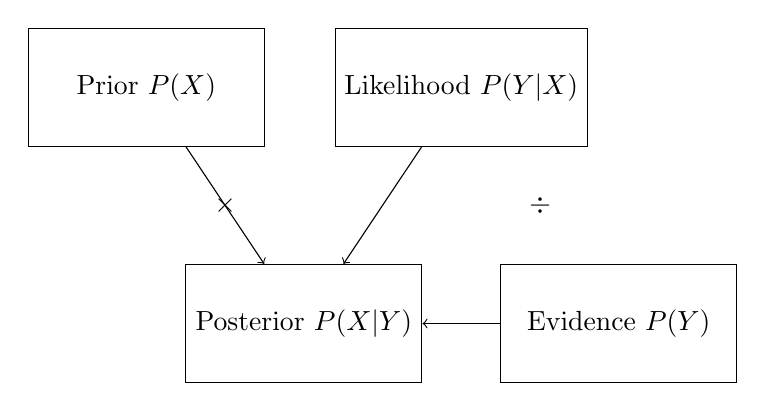
\begin{tikzpicture}
\node[draw, rectangle, minimum width=3cm, minimum height=1.5cm] (prior) at (0,0) {Prior $P(X)$};
\node[draw, rectangle, minimum width=3cm, minimum height=1.5cm] (likelihood) at (4,0) {Likelihood $P(Y|X)$};
\node[draw, rectangle, minimum width=3cm, minimum height=1.5cm] (posterior) at (2,-3) {Posterior $P(X|Y)$};
\node[draw, rectangle, minimum width=3cm, minimum height=1.5cm] (evidence) at (6,-3) {Evidence $P(Y)$};

\draw[->] (prior) -- (posterior);
\draw[->] (likelihood) -- (posterior);
\draw[->] (evidence) -- (posterior);

\node at (1,-1.5) {$\times$};
\node at (5,-1.5) {$\div$};
\end{tikzpicture}
\caption{Bayes' theorem as a belief update process}
\label{fig:bayes-process}
\end{figure}

The formula can be read as: "Posterior = (Likelihood × Prior) ÷ Evidence"

\subsection{Application to Machine Learning}

Bayes' theorem forms the basis of:
\begin{itemize}
    \item Bayesian inference
    \item Naive Bayes classifiers
    \item Maximum a posteriori (MAP) estimation
    \item Bayesian neural networks
\end{itemize}

Given data $\mathcal{D}$ and model parameters $\theta$:

\begin{equation}
P(\theta|\mathcal{D}) = \frac{P(\mathcal{D}|\theta)P(\theta)}{P(\mathcal{D})}
\end{equation}

% Chapter 3, Section 3: Expectation, Variance, and Covariance

\section{Expectation, Variance, and Covariance \difficultyInline{beginner}}
\label{sec:expectation-variance}

\subsection{Intuition: Characterizing Random Variables}

When we have a random variable, we often want to summarize its behavior with a few key numbers:
\begin{itemize}
    \item \textbf{Expected value (mean)}: The "center" or "typical" value
    \item \textbf{Variance}: How much the values spread out from the center
    \item \textbf{Covariance}: How two variables move together
\end{itemize}

Think of it like describing a person:
\begin{itemize}
    \item \textbf{Mean height}: The average height of people in a group
    \item \textbf{Variance in height}: How much heights vary (tall vs short people)
    \item \textbf{Covariance of height and weight}: Do taller people tend to weigh more?
\end{itemize}

\subsection{Expectation}

The \textbf{expected value} or \textbf{mean} of a function $f(x)$ with respect to distribution $P(x)$ is:

For discrete variables:
\begin{equation}
\mathbb{E}_{x \sim P}[f(x)] = \sum_{x} P(x) f(x)
\end{equation}

For continuous variables:
\begin{equation}
\mathbb{E}_{x \sim p}[f(x)] = \int p(x) f(x) \, dx
\end{equation}

\subsubsection{Example: Expected Value of Dice}

For a fair six-sided die:
\begin{align}
\mathbb{E}[X] &= \sum_{x=1}^{6} x \cdot P(X=x) \\
&= 1 \cdot \frac{1}{6} + 2 \cdot \frac{1}{6} + \cdots + 6 \cdot \frac{1}{6} \\
&= \frac{1+2+3+4+5+6}{6} = \frac{21}{6} = 3.5
\end{align}

The expected value is 3.5, even though we can never actually roll 3.5!

\begin{figure}[h]
\centering
\begin{tikzpicture}
\begin{axis}[
    ybar,
    ylabel={Probability},
    xlabel={Dice Value},
    xtick={1,2,3,4,5,6},
    ymin=0,
    ymax=0.2,
    width=10cm,
    height=6cm
]
\addplot coordinates {(1,1/6) (2,1/6) (3,1/6) (4,1/6) (5,1/6) (6,1/6)};
\draw[bookred, thick] (axis cs:3.5,0) -- (axis cs:3.5,0.2);
\node[bookred] at (axis cs:3.5,0.18) {$\mathbb{E}[X] = 3.5$};
\end{axis}
\end{tikzpicture}
\caption{Probability distribution of a fair die with expected value marked}
\label{fig:dice-expectation}
\end{figure}

\subsection{Variance}

\subsubsection{Intuition: Measuring Spread}

Variance tells us how "spread out" the values are around the mean. Think of two dart players:
\begin{itemize}
    \item \textbf{Low variance}: All darts cluster tightly around the bullseye
    \item \textbf{High variance}: Darts are scattered all over the board
\end{itemize}

The \textbf{variance} measures the spread of a distribution:

\begin{equation}
\text{Var}(X) = \mathbb{E}[(X - \mathbb{E}[X])^2] = \mathbb{E}[X^2] - (\mathbb{E}[X])^2
\end{equation}

The \textbf{standard deviation} is $\sigma = \sqrt{\text{Var}(X)}$.

\subsubsection{Example: Variance of Dice}

For our fair die:
\begin{align}
\text{Var}(X) &= \mathbb{E}[X^2] - (\mathbb{E}[X])^2 \\
&= \left(\frac{1^2 + 2^2 + \cdots + 6^2}{6}\right) - (3.5)^2 \\
&= \frac{91}{6} - 12.25 = 15.17 - 12.25 = 2.92
\end{align}

So $\sigma = \sqrt{2.92} \approx 1.71$.

\begin{figure}[h]
\centering
\begin{tikzpicture}
\begin{axis}[
    ybar,
    ylabel={Probability},
    xlabel={Dice Value},
    xtick={1,2,3,4,5,6},
    ymin=0,
    ymax=0.2,
    width=10cm,
    height=6cm
]
\addplot coordinates {(1,1/6) (2,1/6) (3,1/6) (4,1/6) (5,1/6) (6,1/6)};
\draw[bookred, thick] (axis cs:3.5,0) -- (axis cs:3.5,0.2);
\node[bookred] at (axis cs:3.5,0.18) {$\mu = 3.5$};
\draw[bookpurple, thick, <->] (axis cs:1.79,0.1) -- (axis cs:5.21,0.1);
\node[bookpurple] at (axis cs:3.5,0.12) {$\sigma \approx 1.71$};
\end{axis}
\end{tikzpicture}
\caption{Probability distribution showing mean and standard deviation}
\label{fig:dice-variance}
\end{figure}

\subsection{Covariance}

\subsubsection{Intuition: How Variables Move Together}

Covariance tells us whether two variables tend to move in the same direction or opposite directions:
\begin{itemize}
    \item \textbf{Positive covariance}: When one goes up, the other tends to go up too
    \item \textbf{Negative covariance}: When one goes up, the other tends to go down
    \item \textbf{Zero covariance}: No clear relationship
\end{itemize}

Examples:
\begin{itemize}
    \item \textbf{Height and weight}: Positive covariance (taller people tend to weigh more)
    \item \textbf{Price and demand}: Negative covariance (higher prices usually mean lower demand)
    \item \textbf{Height and IQ}: Near zero covariance (no clear relationship)
\end{itemize}

The \textbf{covariance} measures how two variables vary together:

\begin{equation}
\text{Cov}(X, Y) = \mathbb{E}[(X - \mathbb{E}[X])(Y - \mathbb{E}[Y])]
\end{equation}

Positive covariance indicates that $X$ and $Y$ tend to increase together, while negative covariance indicates they tend to vary in opposite directions.

\subsubsection{Example: Height and Weight}

Consider a small dataset of people:
\begin{center}
\begin{tabular}{|c|c|}
\hline
Height (cm) & Weight (kg) \\
\hline
152 & 54 \\
165 & 64 \\
178 & 73 \\
191 & 82 \\
\hline
\end{tabular}
\end{center}

The means are $\mu_X = 171.5$ and $\mu_Y = 68.25$. The covariance is:
\begin{align}
\text{Cov}(X,Y) &= \frac{1}{4}\sum_{i=1}^{4}(x_i - 171.5)(y_i - 68.25) \\
&= \frac{1}{4}[(-19.5)(-14.25) + (-6.5)(-4.25) + (6.5)(4.75) + (19.5)(13.75)] \\
&= \frac{1}{4}[277.875 + 27.625 + 30.875 + 268.125] = \frac{604.5}{4} = 151.125
\end{align}

Positive covariance confirms that taller people tend to weigh more!

\subsection{Correlation}

The \textbf{correlation coefficient} normalizes covariance:

\begin{equation}
\rho(X, Y) = \frac{\text{Cov}(X, Y)}{\sqrt{\text{Var}(X)\text{Var}(Y)}}
\end{equation}

Properties:
\begin{itemize}
    \item $-1 \leq \rho \leq 1$
    \item $|\rho| = 1$ indicates perfect linear relationship
    \item $\rho = 0$ indicates no linear relationship (but variables may still be dependent)
\end{itemize}

% Chapter 3, Section 4: Common Probability Distributions

\section{Common Probability Distributions \difficultyInline{beginner}}
\label{sec:common-distributions}

Understanding common probability distributions is essential for deep learning because different distributions model different types of data and uncertainty, from binary outcomes in classification tasks to continuous values in regression problems, and from simple univariate cases to complex multivariate scenarios. These distributions provide the mathematical foundation for modeling the behavior of neural network weights, activation functions, and output predictions, enabling us to make principled decisions about model architecture, loss functions, and regularization strategies. By learning these distributions, we can better understand how to design neural networks that can handle various types of data and uncertainty, from the simple Bernoulli distribution for binary classification to the complex multivariate Gaussian for high-dimensional feature representations.

\subsection{Bernoulli Distribution}

Models a binary random variable (0 or 1):

\begin{equation}
P(X=1) = \phi, \quad P(X=0) = 1-\phi
\end{equation}

Used for binary classification problems.

\begin{example}
Consider a biased coin that lands heads with probability 0.7. Let $X$ be the random variable representing the outcome:
\begin{itemize}
    \item $X = 1$ if the coin lands heads
    \item $X = 0$ if the coin lands tails
\end{itemize}

The probability mass function is:
\begin{align}
P(X=1) &= 0.7 \quad \text{(probability of heads)} \\
P(X=0) &= 0.3 \quad \text{(probability of tails)}
\end{align}

The expected value is $\mathbb{E}[X] = 1 \cdot 0.7 + 0 \cdot 0.3 = 0.7$, and the variance is $\text{Var}(X) = 0.7 \cdot 0.3 = 0.21$.
\end{example}

\subsection{Categorical Distribution}

Generalizes Bernoulli to $k$ discrete outcomes. If $X$ can take values $\{1, 2, \ldots, k\}$:

\begin{equation}
P(X=i) = p_i \quad \text{where} \quad \sum_{i=1}^{k} p_i = 1
\end{equation}

\subsection{Gaussian (Normal) Distribution}

The Gaussian or normal distribution is the most important continuous distribution in deep learning, characterized by its bell-shaped curve and defined by its mean $\mu$ and variance $\sigma^2$. This distribution is particularly important because of the central limit theorem, which states that sums of independent variables approach a Gaussian distribution, making it a natural choice for modeling many real-world phenomena and neural network activations. The Gaussian distribution has several key properties that make it useful in deep learning: it has a single peak at the mean, it's symmetric around the mean, and it has the property that about 68% of the data falls within one standard deviation of the mean, 95% within two standard deviations, and 99.7% within three standard deviations.

The multivariate Gaussian with mean vector $\boldsymbol{\mu}$ and covariance matrix $\boldsymbol{\Sigma}$ is:

\begin{equation}
\mathcal{N}(\vect{x}; \boldsymbol{\mu}, \boldsymbol{\Sigma}) = \frac{1}{\sqrt{(2\pi)^n |\boldsymbol{\Sigma}|}} \exp\left(-\frac{1}{2}(\vect{x}-\boldsymbol{\mu})^\top \boldsymbol{\Sigma}^{-1} (\vect{x}-\boldsymbol{\mu})\right)
\end{equation}

\begin{figure}[h]
\centering
\begin{tikzpicture}
\begin{axis}[
    ylabel={Probability Density},
    xlabel={Value},
    domain=-4:4,
    width=10cm,
    height=6cm,
    samples=100,
    grid=major,
    grid style={line width=.1pt, draw=gray!10},
    major grid style={line width=.2pt, draw=gray!50}
]
\addplot[bookpurple, thick] {1/sqrt(2*pi) * exp(-x^2/2)};
\node[bookpurple] at (axis cs:0,0.4) {$\mathcal{N}(0, 1)$};
\end{axis}
\end{tikzpicture}
\caption{Gaussian (Normal) distribution with mean $\mu = 0$ and standard deviation $\sigma = 1$. This is the standard normal distribution, which is commonly used as a reference in statistics and machine learning.}
\label{fig:gaussian-distribution}
\end{figure}

\subsection{Exponential Distribution}

Models the time between events in a Poisson process:

\begin{equation}
p(x; \lambda) = \lambda e^{-\lambda x} \quad \text{for } x \geq 0
\end{equation}

\begin{figure}[h]
\centering
\begin{tikzpicture}
\begin{axis}[
    ylabel={Probability Density},
    xlabel={Value},
    domain=0:5,
    width=10cm,
    height=6cm,
    samples=100,
    grid=major,
    grid style={line width=.1pt, draw=gray!10},
    major grid style={line width=.2pt, draw=gray!50}
]
\addplot[bookred, thick] {exp(-x)};
\node[bookred] at (axis cs:1,0.3) {$\lambda = 1$};
\end{axis}
\end{tikzpicture}
\caption{Exponential distribution with rate parameter $\lambda = 1$. The distribution starts at its maximum value and decreases exponentially.}
\label{fig:exponential-distribution}
\end{figure}

\subsection{Laplace Distribution}

Heavy-tailed alternative to Gaussian:

\begin{equation}
\text{Laplace}(x; \mu, b) = \frac{1}{2b} \exp\left(-\frac{|x-\mu|}{b}\right)
\end{equation}

Used in robust statistics and L1 regularization.

\begin{figure}[h]
\centering
\begin{tikzpicture}
\begin{axis}[
    ylabel={Probability Density},
    xlabel={Value},
    domain=-4:4,
    width=10cm,
    height=6cm,
    samples=100,
    grid=major,
    grid style={line width=.1pt, draw=gray!10},
    major grid style={line width=.2pt, draw=gray!50}
]
\addplot[bookpurple, thick] {0.5 * exp(-abs(x))};
\node[bookpurple] at (axis cs:0,0.4) {$\mu = 0, b = 1$};
\end{axis}
\end{tikzpicture}
\caption{Laplace distribution with location parameter $\mu = 0$ and scale parameter $b = 1$. The distribution has a sharp peak at the mean and exponential tails, making it more robust to outliers than the Gaussian distribution.}
\label{fig:laplace-distribution}
\end{figure}

\subsection{Dirac Delta and Mixture Distributions}

The \textbf{Dirac delta} $\delta(x)$ concentrates all probability at a single point:

\begin{equation}
p(x) = \delta(x - \mu)
\end{equation}

\textbf{Mixture distributions} combine multiple distributions:

\begin{equation}
p(x) = \sum_{i=1}^{k} \alpha_i p_i(x), \quad \sum_{i=1}^{k} \alpha_i = 1
\end{equation}

\begin{example}[Gaussian Mixture Model (GMM)]
A Gaussian Mixture Model is a probabilistic model that represents a probability distribution as a weighted sum of multiple Gaussian distributions, allowing it to model complex, multi-modal data that cannot be captured by a single Gaussian. GMMs are particularly useful in clustering, density estimation, and as building blocks for more complex generative models in deep learning.

The probability density function of a GMM with $K$ components is:
\begin{equation}
p(\vect{x}) = \sum_{k=1}^{K} \pi_k \mathcal{N}(\vect{x}; \boldsymbol{\mu}_k, \boldsymbol{\Sigma}_k)
\end{equation}

where:
\begin{itemize}
    \item $\pi_k$ are the mixing weights (probabilities) satisfying $\sum_{k=1}^{K} \pi_k = 1$
    \item $\boldsymbol{\mu}_k$ and $\boldsymbol{\Sigma}_k$ are the mean and covariance matrix of the $k$-th Gaussian component
    \item $\mathcal{N}(\vect{x}; \boldsymbol{\mu}_k, \boldsymbol{\Sigma}_k)$ is the multivariate Gaussian density function
\end{itemize}

The key insight is that each data point $\vect{x}$ can be thought of as being generated by first selecting one of the $K$ Gaussian components according to the mixing weights $\pi_k$, and then sampling from that selected component. This allows the model to capture complex, multi-modal distributions that arise naturally in real-world data, such as images with multiple object classes or speech signals with different phonemes.
\end{example}

% Chapter 3, Section 5: Information Theory Basics

\section{Information Theory Basics \difficultyInline{beginner}}
\label{sec:information-theory}

Information theory provides tools for quantifying information and uncertainty, which are crucial for understanding learning and compression.

\subsection{Self-Information}

The \textbf{self-information} or \textbf{surprisal} of an event $x$ is:

\begin{equation}
I(x) = -\log P(x)
\end{equation}

Rare events have high information content, while certain events have zero information.

\subsection{Entropy}

The \textbf{Shannon entropy} measures the expected information in a distribution:

\begin{equation}
H(X) = \mathbb{E}_{x \sim P}[I(x)] = -\sum_{x} P(x) \log P(x)
\end{equation}

For continuous distributions, we use \textbf{differential entropy}:

\begin{equation}
H(X) = -\int p(x) \log p(x) \, dx
\end{equation}

Entropy is maximized when all outcomes are equally likely.

\subsection{Cross-Entropy}

The \textbf{cross-entropy} between distributions $P$ and $Q$ is:

\begin{equation}
H(P, Q) = -\mathbb{E}_{x \sim P}[\log Q(x)] = -\sum_{x} P(x) \log Q(x)
\end{equation}

In deep learning, cross-entropy is commonly used as a loss function for classification.

\subsection{Kullback-Leibler Divergence}

The \textbf{KL divergence} measures how one distribution differs from another:

\begin{equation}
D_{KL}(P \| Q) = \mathbb{E}_{x \sim P}\left[\log \frac{P(x)}{Q(x)}\right] = \sum_{x} P(x) \log \frac{P(x)}{Q(x)}
\end{equation}

Properties:
\begin{itemize}
    \item $D_{KL}(P \| Q) \geq 0$ with equality if and only if $P = Q$
    \item Not symmetric: $D_{KL}(P \| Q) \neq D_{KL}(Q \| P)$
    \item Related to cross-entropy: $D_{KL}(P \| Q) = H(P, Q) - H(P)$
\end{itemize}

\subsection{Mutual Information}

The \textbf{mutual information} between $X$ and $Y$ quantifies how much knowing one reduces uncertainty about the other:

\begin{equation}
I(X; Y) = D_{KL}(P(X, Y) \| P(X)P(Y))
\end{equation}

Equivalently:

\begin{equation}
I(X; Y) = H(X) - H(X|Y) = H(Y) - H(Y|X)
\end{equation}

Mutual information is symmetric and measures the dependence between variables.

\subsection{Applications in Deep Learning}

Information theory concepts are used in:
\begin{itemize}
    \item Loss functions (cross-entropy loss)
    \item Model selection (AIC, BIC use information-theoretic principles)
    \item Variational inference (minimizing KL divergence)
    \item Information bottleneck theory
    \item Mutual information maximization in self-supervised learning
\end{itemize}

% % Chapter 3, Section 6: Problems

\section{Problems \difficultyInline{beginner}}
\label{sec:probability-problems}

This section provides exercises to reinforce your understanding of probability and information theory concepts. Problems are categorized by difficulty level.

\subsection{Easy Problems (6 problems)}

\begin{problem}[Coin Flipping]
A fair coin is flipped 3 times. What is the probability of getting exactly 2 heads?
\end{problem}

\begin{problem}[Dice Probability]
A fair six-sided die is rolled. What is the probability of getting an even number?
\end{problem}

\begin{problem}[Basic Conditional Probability]
In a class of 30 students, 18 are girls and 12 are boys. If a student is selected at random, what is the probability that they are a girl?
\end{problem}

\begin{problem}[Independent Events]
Two fair coins are flipped. What is the probability that both show heads?
\end{problem}

\begin{problem}[Complement Rule]
The probability that it will rain tomorrow is 0.3. What is the probability that it will not rain tomorrow?
\end{problem}

\begin{problem}[Basic Expectation]
A fair die is rolled. What is the expected value of the outcome?
\end{problem}

\subsection{Medium Problems (5 problems)}

\begin{problem}[Bayes' Theorem Application]
A medical test for a disease has a 95\% accuracy rate (sensitivity) and a 90\% specificity rate. If 2\% of the population has the disease, what is the probability that a person who tests positive actually has the disease?
\end{problem}

\begin{problem}[Joint Probability]
In a survey of 100 people, 60 like pizza, 40 like burgers, and 20 like both. If a person is selected at random, what is the probability that they like pizza or burgers (or both)?
\end{problem}

\begin{problem}[Variance Calculation]
A random variable $X$ has the following probability distribution:
\begin{center}
\begin{tabular}{|c|c|}
\hline
$x$ & $P(X=x)$ \\
\hline
1 & 0.2 \\
2 & 0.3 \\
3 & 0.3 \\
4 & 0.2 \\
\hline
\end{tabular}
\end{center}
Calculate the variance of $X$.
\end{problem}

\begin{problem}[Normal Distribution]
A random variable $X$ follows a normal distribution with mean $\mu = 50$ and standard deviation $\sigma = 10$. What is the probability that $X$ is between 40 and 60?
\end{problem}

\begin{problem}[Entropy Calculation]
A random variable $X$ can take values $\{1, 2, 3, 4\}$ with probabilities $\{0.1, 0.4, 0.3, 0.2\}$ respectively. Calculate the entropy $H(X)$.
\end{problem}

\subsection{Hard Problems (5 problems)}

\begin{problem}[Bayesian Inference]
You have two coins: one fair and one biased (with probability 0.8 of heads). You randomly select one coin and flip it 3 times, getting heads each time. What is the probability that you selected the biased coin?
\end{problem}

\begin{problem}[Covariance and Correlation]
Two random variables $X$ and $Y$ have the following joint probability distribution:
\begin{center}
\begin{tabular}{|c|c|c|}
\hline
 & $Y=1$ & $Y=2$ \\
\hline
$X=1$ & 0.2 & 0.1 \\
$X=2$ & 0.3 & 0.4 \\
\hline
\end{tabular}
\end{center}
Calculate the covariance and correlation coefficient between $X$ and $Y$.
\end{problem}

\begin{problem}[KL Divergence]
Calculate the Kullback-Leibler divergence $D_{KL}(P \| Q)$ where:
\begin{align}
P(x) &= \begin{cases} 0.5 & \text{if } x = 0 \\ 0.5 & \text{if } x = 1 \end{cases} \\
Q(x) &= \begin{cases} 0.3 & \text{if } x = 0 \\ 0.7 & \text{if } x = 1 \end{cases}
\end{align}
\end{problem}

\begin{problem}[Mutual Information]
Two random variables $X$ and $Y$ have joint distribution:
\begin{center}
\begin{tabular}{|c|c|c|}
\hline
 & $Y=0$ & $Y=1$ \\
\hline
$X=0$ & 0.4 & 0.1 \\
$X=1$ & 0.2 & 0.3 \\
\hline
\end{tabular}
\end{center}
Calculate the mutual information $I(X; Y)$.
\end{problem}

\begin{problem}[Maximum Likelihood and MAP]
Given observations $\{x_1, x_2, \ldots, x_n\}$ from a normal distribution $\mathcal{N}(\mu, \sigma^2)$, derive the maximum likelihood estimate of $\mu$. Then, assuming a normal prior $\mathcal{N}(\mu_0, \sigma_0^2)$ for $\mu$, derive the MAP estimate.
\end{problem}

\section*{Hints}

\subsection*{Easy Problems Hints}

\begin{enumerate}
\item \textbf{Coin Flipping}: Use the binomial distribution or enumerate all possible outcomes.
\item \textbf{Dice Probability}: Count favorable outcomes (2, 4, 6) over total outcomes.
\item \textbf{Basic Conditional Probability}: This is just a ratio of favorable cases to total cases.
\item \textbf{Independent Events}: Multiply the individual probabilities.
\item \textbf{Complement Rule}: Use $P(\text{not A}) = 1 - P(A)$.
\item \textbf{Basic Expectation}: Use the definition $\mathbb{E}[X] = \sum x \cdot P(X=x)$.
\end{enumerate}

\subsection*{Medium Problems Hints}

\begin{enumerate}
\item \textbf{Bayes' Theorem}: Use the formula $P(\text{Disease}|\text{Positive}) = \frac{P(\text{Positive}|\text{Disease})P(\text{Disease})}{P(\text{Positive})}$.
\item \textbf{Joint Probability}: Use the inclusion-exclusion principle: $P(A \cup B) = P(A) + P(B) - P(A \cap B)$.
\item \textbf{Variance Calculation}: First find $\mathbb{E}[X]$ and $\mathbb{E}[X^2]$, then use $\text{Var}(X) = \mathbb{E}[X^2] - (\mathbb{E}[X])^2$.
\item \textbf{Normal Distribution}: Use the 68-95-99.7 rule or standardize and use normal tables.
\item \textbf{Entropy Calculation}: Use $H(X) = -\sum_{i} p_i \log p_i$.
\end{enumerate}

\subsection*{Hard Problems Hints}

\begin{enumerate}
\item \textbf{Bayesian Inference}: Use Bayes' theorem with the prior probability of selecting each coin.
\item \textbf{Covariance and Correlation}: First find marginal distributions, then use $\text{Cov}(X,Y) = \mathbb{E}[XY] - \mathbb{E}[X]\mathbb{E}[Y]$.
\item \textbf{KL Divergence}: Use $D_{KL}(P \| Q) = \sum_x P(x) \log \frac{P(x)}{Q(x)}$.
\item \textbf{Mutual Information}: Use $I(X;Y) = H(X) + H(Y) - H(X,Y)$ or $I(X;Y) = \sum_{x,y} P(x,y) \log \frac{P(x,y)}{P(x)P(y)}$.
\item \textbf{Maximum Likelihood and MAP}: Take derivatives of the log-likelihood and log-posterior respectively.
\end{enumerate}


% Chapter summary and problems
% Key Takeaways for Chapter 3

\section*{Key Takeaways}
\addcontentsline{toc}{section}{Key Takeaways}

\begin{keytakeaways}
\begin{itemize}[leftmargin=2em]
    \item \textbf{Probability distributions} model uncertainty and enable principled reasoning under incomplete information.
    \item \textbf{Bayes' theorem} provides a framework for updating beliefs with evidence, central to many machine learning algorithms.
    \item \textbf{Expectation and variance} characterise random variables and guide choices of loss functions and model architectures.
    \item \textbf{Common distributions} (Bernoulli, Gaussian, categorical) serve as building blocks for probabilistic models.
    \item \textbf{Information theory} quantifies uncertainty through entropy and divergence, directly connecting to loss functions and regularisation.
\end{itemize}
\end{keytakeaways}



% Exercises (Hands-On Exercises) for Chapter 3: Probability and Information Theory

\section*{Exercises}
\addcontentsline{toc}{section}{Exercises}

\subsection*{Easy}

\begin{problem}[Bayes' Theorem Application]
Given that P(Disease) = 0.01, P(Positive Test | Disease) = 0.95, and P(Positive Test | No Disease) = 0.05, calculate P(Disease | Positive Test).

\textbf{Hint:} Use Bayes' theorem: $P(A|B) = \frac{P(B|A)P(A)}{P(B)}$. Remember to compute P(Positive Test) first.
\end{problem}

\begin{problem}[Expectation and Variance]
A discrete random variable $X$ takes values 1, 2, 3, 4 with probabilities 0.1, 0.2, 0.4, 0.3 respectively. Calculate $\mathbb{E}[X]$ and $\text{Var}(X)$.

\textbf{Hint:} $\mathbb{E}[X] = \sum_i x_i P(X=x_i)$ and $\text{Var}(X) = \mathbb{E}[X^2] - (\mathbb{E}[X])^2$.
\end{problem}

\begin{problem}[Entropy Calculation]
Calculate the entropy of a fair coin flip and compare it to the entropy of a biased coin with P(Heads) = 0.9.

\textbf{Hint:} Entropy $H(X) = -\sum_i p_i \log_2 p_i$. Higher entropy means more uncertainty.
\end{problem}

\begin{problem}[Independence Test]
Given P(A) = 0.3, P(B) = 0.4, and P(A $\cap$ B) = 0.12, determine if events A and B are independent.

\textbf{Hint:} Events are independent if P(A $\cap$ B) = P(A)P(B).
\end{problem}

\begin{problem}[Conditional Probability]
In a deck of 52 cards, what is the probability of drawing a heart given that the card drawn is red?

\textbf{Hint:} Use the definition of conditional probability: P(A|B) = P(A $\cap$ B)/P(B).
\end{problem}

\begin{problem}[Joint Probability]
Given P(A) = 0.6, P(B) = 0.4, and P(A|B) = 0.8, find P(A $\cap$ B) and P(B|A).

\textbf{Hint:} Use the multiplication rule: P(A $\cap$ B) = P(A|B)P(B).
\end{problem}

\begin{problem}[Probability Distributions]
A random variable X follows a uniform distribution on [0, 2]. Find P(X > 1.5) and the expected value E[X].

\textbf{Hint:} For uniform distribution on [a, b], the density is f(x) = 1/(b-a) for x in [a, b].
\end{problem}

\begin{problem}[Binomial Distribution]
A fair coin is flipped 10 times. What is the probability of getting exactly 7 heads?

\textbf{Hint:} Use the binomial probability formula: $P(X = k) = C(n,k) p^k (1-p)^{(n-k)}$.
\end{problem}

\begin{problem}[Normal Distribution]
If X ~ N(50, 25), find P(45 < X < 55) using the standard normal distribution.

\textbf{Hint:} Standardise using Z = (X - μ)/σ, then use standard normal tables.
\end{problem}

\begin{problem}[Information Content]
Calculate the information content of an event with probability 0.1, and compare it to an event with probability 0.5.

\textbf{Hint:} Information content is I(x) = -log₂ P(x).
\end{problem}

\begin{problem}[Mutual Information]
Given P(X=0) = 0.6, P(X=1) = 0.4, P(Y=0|X=0) = 0.8, P(Y=1|X=0) = 0.2, P(Y=0|X=1) = 0.3, P(Y=1|X=1) = 0.7, calculate I(X;Y).

\textbf{Hint:} Use I(X;Y) = H(X) - H(X|Y) = H(Y) - H(Y|X).
\end{problem}

\subsection*{Medium}

\begin{problem}[KL Divergence for Model Comparison]
Explain why Kullback-Leibler (KL) divergence is not symmetric and discuss its implications when comparing probability distributions in machine learning.

\textbf{Hint:} Consider $D_{KL}(P||Q)$ versus $D_{KL}(Q||P)$ and their behaviour when $P$ or $Q$ is close to zero.
\end{problem}

\begin{problem}[Cross-Entropy Loss]
Show that minimising cross-entropy loss is equivalent to maximising the log-likelihood for classification tasks. Derive the relationship mathematically.

\textbf{Hint:} Start with the cross-entropy $H(p,q) = -\sum_i p_i \log q_i$ where $p$ is the true distribution and $q$ is the predicted distribution.
\end{problem}

\begin{problem}[Maximum Likelihood Estimation]
Given a sample of n independent observations from a normal distribution N(μ, σ²), derive the maximum likelihood estimators for μ and σ².

\textbf{Hint:} Write the likelihood function L(μ, σ²) and take partial derivatives with respect to μ and σ².
\end{problem}

\begin{problem}[Jensen's Inequality Application]
Use Jensen's inequality to show that the entropy of a mixture of distributions is at least the weighted average of the individual entropies.

\textbf{Hint:} Consider H(∑ᵢ αᵢpᵢ) ≥ ∑ᵢ αᵢH(pᵢ) where ∑ᵢ αᵢ = 1 and αᵢ ≥ 0.
\end{problem}

\begin{problem}[Central Limit Theorem]
Explain how the Central Limit Theorem applies to the convergence of sample means and discuss its implications for machine learning.

\textbf{Hint:} Consider the distribution of sample means and how it approaches normality regardless of the original distribution.
\end{problem}

\begin{problem}[Concentration Inequalities]
Use Markov's inequality to bound P(X ≥ 2E[X]) for a non-negative random variable X, and compare with Chebyshev's inequality.

\textbf{Hint:} Markov's inequality: P(X ≥ a) ≤ E[X]/a for a > 0.
\end{problem}

\begin{problem}[Bayesian Inference]
Given a prior Beta(2, 2) distribution and observing 7 successes in 10 trials, find the posterior distribution and the Bayesian estimate.

\textbf{Hint:} Use the Beta-Binomial conjugate relationship: Beta(α, β) + Binomial(n, p) → Beta(α + k, β + n - k).
\end{problem}

\subsection*{Hard}

\begin{problem}[Information Theory in Neural Networks]
Analyse how mutual information between layers in a neural network can be used to understand information flow during training. Discuss the information bottleneck principle.

\textbf{Hint:} Consider $I(X;Y) = H(X) - H(X|Y)$ and how it relates to representation learning.
\end{problem}

\begin{problem}[Variational Inference]
Derive the Evidence Lower Bound (ELBO) for variational inference and explain its relationship to the Kullback-Leibler divergence.

\textbf{Hint:} Start with log p(x) = log ∫ p(x,z) dz and use Jensen's inequality with a variational distribution q(z).
\end{problem}

\begin{problem}[Information Bottleneck Theory]
Prove that the information bottleneck principle leads to a trade-off between compression and prediction accuracy in representation learning.

\textbf{Hint:} Consider the Lagrangian L = I(X;T) - βI(T;Y) where T is the representation and β controls the trade-off.
\end{problem}

\begin{problem}[PAC-Bayes Bounds]
Derive a PAC-Bayes bound for generalisation error in terms of the KL divergence between prior and posterior distributions.

\textbf{Hint:} Use the change of measure inequality and the union bound over the hypothesis space.
\end{problem}

\begin{problem}[Maximum Entropy Principle]
Show that the maximum entropy distribution under moment constraints is exponential family, and derive the dual optimisation problem.

\textbf{Hint:} Use Lagrange multipliers to maximise H(p) subject to E[φᵢ(X)] = μᵢ for moment constraints.
\end{problem}

\begin{problem}[Causal Inference and Information Theory]
Analyse the relationship between causal discovery and information-theoretic measures, particularly in the context of conditional independence testing.

\textbf{Hint:} Consider how mutual information relates to conditional independence: X ⊥ Y | Z if and only if I(X;Y|Z) = 0.
\end{problem}


